\documentclass[10pt]{article}
\usepackage[paperwidth=198mm,paperheight=59mm,margin=1mm]{geometry}
\usepackage{newtxtext,newtxmath,tikz,pgfplots}
\pgfplotsset{compat=1.18}
\definecolor{methodblue}{HTML}{216A85}
\definecolor{controlgray}{HTML}{555555}
\definecolor{accentorange}{HTML}{A64B1D}
\pagestyle{empty}
\begin{document}\noindent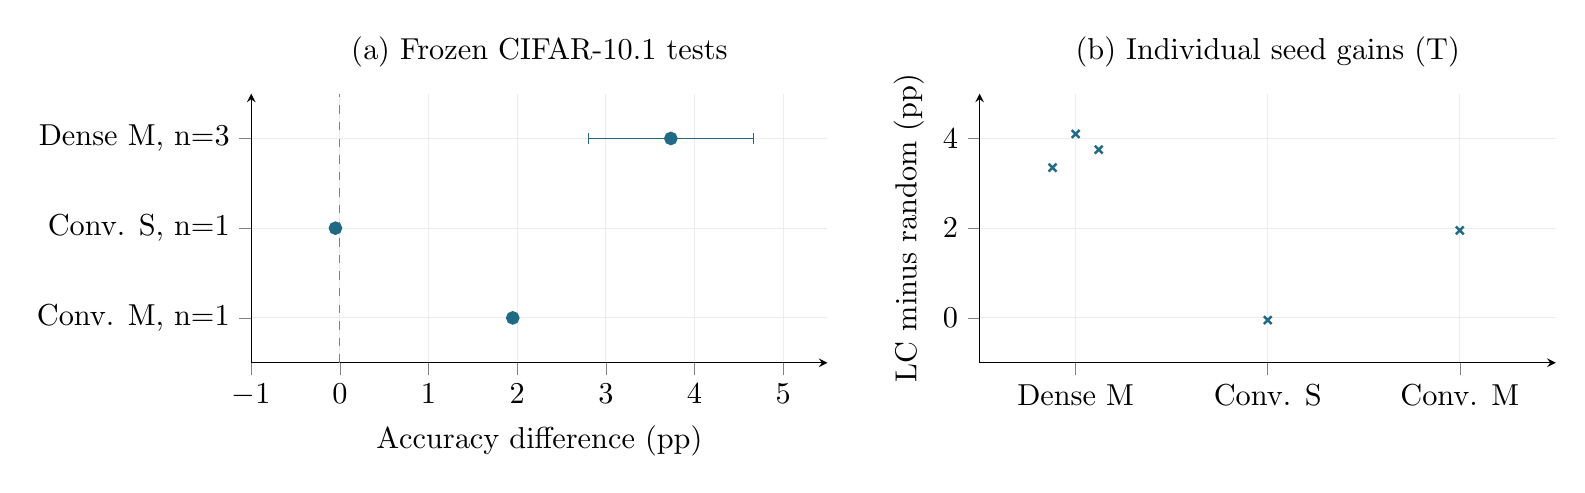
\begin{tikzpicture}
\begin{axis}[width=89mm,height=50mm,axis lines=left,tick align=outside,grid=major,grid style={gray!15},scaled ticks=false,tick label style={font=\fontsize{11}{13}\selectfont},label style={font=\fontsize{11}{13}\selectfont},title style={font=\fontsize{11}{13}\selectfont},legend style={font=\fontsize{11}{13}\selectfont,draw=none,fill=white,inner sep=1pt},title={(a) Frozen CIFAR-10.1 tests},xmin=-1,xmax=5.5,ymin=-.5,ymax=2.5,ytick={0,1,2},yticklabels={{Conv. M, n=1},{Conv. S, n=1},{Dense M, n=3}},xlabel={Accuracy difference (pp)}]
\draw[dashed,gray] (axis cs:0,-.5)--(axis cs:0,2.5);
\addplot+[color=methodblue,mark=*,mark size=2pt,line width=0.9pt,mark options={solid,fill=methodblue,draw=methodblue},only marks,error bars/.cd,x dir=both,x explicit] coordinates {(3.7333333,2) +- (0.93231667,0)};
\addplot+[color=methodblue,mark=*,mark size=2pt,line width=0.9pt,mark options={solid,fill=methodblue,draw=methodblue},only marks] coordinates {(-0.05,1)};
\addplot+[color=methodblue,mark=*,mark size=2pt,line width=0.9pt,mark options={solid,fill=methodblue,draw=methodblue},only marks] coordinates {(1.95,0)};
\end{axis}
\begin{axis}[width=89mm,height=50mm,axis lines=left,tick align=outside,grid=major,grid style={gray!15},scaled ticks=false,tick label style={font=\fontsize{11}{13}\selectfont},label style={font=\fontsize{11}{13}\selectfont},title style={font=\fontsize{11}{13}\selectfont},legend style={font=\fontsize{11}{13}\selectfont,draw=none,fill=white,inner sep=1pt},at={(9.25cm,0)},anchor=south west,title={(b) Individual seed gains (T)},xmin=-.5,xmax=2.5,ymin=-1,ymax=5,xtick={0,1,2},xticklabels={Dense M,Conv. S,Conv. M},ylabel={LC minus random (pp)}]
\addplot+[color=methodblue,mark=x,mark size=2pt,line width=0.9pt,mark options={solid,fill=methodblue,draw=methodblue},only marks] coordinates {(-0.12,3.35)(0,4.1)(0.12,3.75)};
\addplot+[color=methodblue,mark=x,mark size=2pt,line width=0.9pt,mark options={solid,fill=methodblue,draw=methodblue},only marks] coordinates {(1,-0.05)};
\addplot+[color=methodblue,mark=x,mark size=2pt,line width=0.9pt,mark options={solid,fill=methodblue,draw=methodblue},only marks] coordinates {(2,1.95)};
\end{axis}
\end{tikzpicture}\end{document}
